\apendice{Documentación de usuario}

\section{Introducción}\label{manualusuario}
En este apartado se recoge todo lo que un usuario necesita conocer para poder ejecutar la aplicación en su teléfono móvil Android personal y los requisitos mínimos necesarios.

\section{Requisitos de usuarios}
Los requerimientos necesarios para poder ejecutar la aplicación en el teléfono son:
\begin{itemize}
	\tightlist
	\item
	Disponer de un terminal que al menos tenga la versión de Android en \emph{Lollipop}. Esto se debe a que cuando se compila la aplicación en Flutter, algunos de los servicios necesitan al menos que el SDK sea el 21~\cite{wiki:versionAndroid}. Limitando por abajo el número de sistemas operativos compatibles.
	\item
	Es necesario disponer de conexión a Internet, tanto como para bajarse la aplicación en \emph{Store}, como para usar los servicios, ya que es necesario logearse con \emph{Google}
	\item La clasificación de contenido, es PEGI 3~\cite{wiki:pegi}. 
	\item En el caso de que la descarga se realice mediante la tienda oficial, los países para los que la aplicación está disponible son: España, Francia, Portugal e Irlanda. En el caso de que no sea así, será necesario descargar desde Github, como se explica en la página~\pageref{descargaGit}.
\end{itemize}

\section{Instalación}
La instalación se puede hacer a través de dos métodos diferentes:

\subsection{GitHub:}\label{descargaGit}
Desde el repositorio donde está el proyecto en el apartado de las \emph{releases}~\cite{github:releases}, podemos encontrar la última de las versiones compiladas, con el fin de descargarla.

Al ser una aplicación de orígenes desconocidos, ya que no se descarga de la tienda se deben de seguir los siguientes pasos para la instalación:
\begin{enumerate}
	\tightlist
	\item Ir a los ajustes del terminal.
	\item Apartado de privacidad o seguridad.
	\item Activar el \emph{slider} de `Orígenes desconocidos''.
	\item Ejecutar el fichero .apk que acabamos de descargar.
	\item Instalar y abrir la aplicación.
\end{enumerate}

\subsection{Play Store:}
La manera más cómoda de hacerlo, es dirigirse \href{https://play.google.com/store/apps/details?id=com.ubu.flutter_snake}{Flutter games}, que es el enlace de descarga para dispositivos móviles Android. La versión disponible es la 6, ya que se han tenido que realizar varias pruebas con el fin de validar la disponibilidad, por eso el número de versión que tiene.



\imagen{manual/tienda.jpg}{Tienda con el proyecto}

El proceso de instalación es simple, solo se tiene que dar al botón de instalar. En el caso de que nos encontremos en el navegador web, deja elegir el dispositivo que tenemos vinculado a nuestra cuenta de \emph{Google}. No sucede lo mismo si nos encontramos desde el terminal, ya se instalará sin ningún problema.

En el caso de que se lancen nuevas versiones del producto, las actualizaciones se realizarán de forma automática, en el caso de estar activadas.

\section{Manual de usuario}
Se pretende mostrar el funcionamiento de cada una de las ventanas que están disponibles en la aplicación, con el fin de poder informar a los usuarios del funcionamiento de cada una de estas.

Las ventanas de las que consta la aplicación son las siguientes:

\begin{itemize}
	\tightlist
	\item Log in~\pageref{login}.
	\item Home~\pageref{home}.
	\item About~\pageref{about}.
	\item Settings~\pageref{settings}.
	\item Menú de juegos~\pageref{menugames}.
	\item Snake~\pageref{snake}.
	\item Ranking~\pageref{rank}.
	\item Cuatro en raya online menú~\pageref{cuatromenu}:.
	\subitem Invitar~\pageref{cuatroinvitar}.
	\subitem Unirse~\pageref{cuatrounir}.
	\subitem Juego~\pageref{cuatrojuego}.
\end{itemize}

\subsection{Log in}\label{login}
Es la primera ventana que nos encontramos cuando lanzamos la aplicación. Es necesario que nos registremos siempre con la cuenta de \emph{Google} que tengamos disponible, ya que muchos de los servicios están en la nube, no esta permitido el acceso mediante anonimato.

\begin{figure}[H]
	\centering
	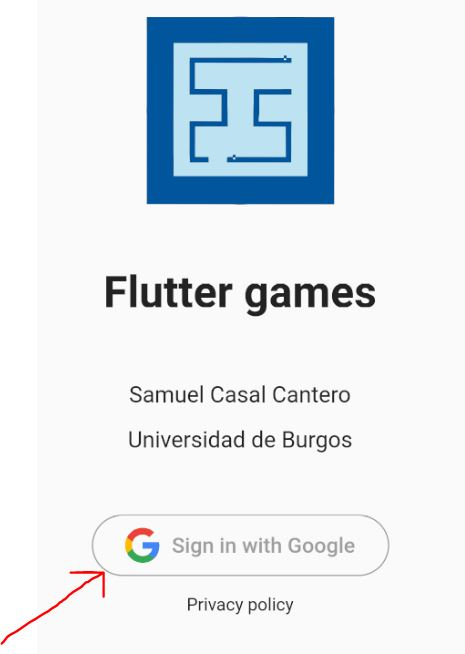
\includegraphics[height=0.7\textwidth]{manual/loginpage.jpg}
	\caption{Log in page}\label{fig:loginpage}
\end{figure}

Cuando pulsamos en el botón de \emph{sign in with Google}, nos aparecerá la ventana siguiente~\ref{fig:formlog}, dónde nos pedirá que ingresemos el usuario de nuestra cuenta de \emph{Google}. También se puede consultar la política de privacidad~\ref{fig:policy}

\begin{figure}[H]
	\centering
	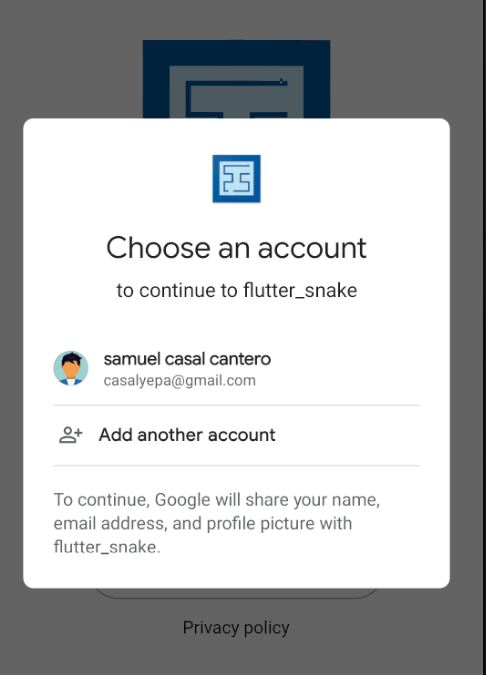
\includegraphics[height=0.7\textwidth]{manual/loginform.jpg}
	\caption{Formulario sign in}\label{fig:formlog}
\end{figure}

\begin{figure}[H]
	\centering
	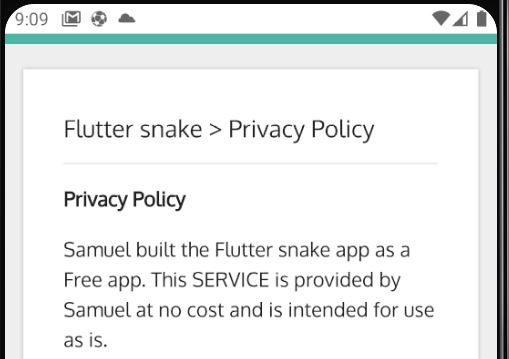
\includegraphics[width=0.7\textwidth]{manual/policy.jpg}
	\caption{Política de privacidad}\label{fig:policy}
\end{figure}

Una vez completemos este proceso, la ventana siguiente a la que nos redirige la aplicación es el Home~\ref{fig:homepage}.


\subsection{Home}\label{home}
Esta página, es donde se muestra el póster del proyecto, además de tener el acceso al menú lateral de la aplicación. Para acceder a este tenemos que deslizar lateralmente a la derecha, y para cerrarlo, tenemos que hacer el proceso inverso deslizando hacia la izquierda o pulsando fuera del menú~\ref{fig:menuhome}. Otra de las formas de entrar a este es pulsando el menú hamburguesa.

\begin{figure}[H]
	\centering
	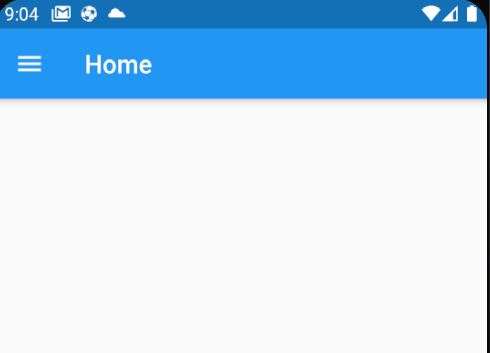
\includegraphics[width=0.7\textwidth]{manual/home.jpg}
	\caption{Home}\label{fig:homepage}
\end{figure}

\begin{figure}[H]
	\centering
	
\includegraphics[width=0.7\textwidth]{manual/banner.jpg}
	\caption{Banner}\label{fig:banner}
\end{figure}

Como podemos ver en la imagen~\ref{fig:banner}, tenemos un \emph{banner} donde se nos muestra la publicidad, en el caso de que pinchemos en el, nos abrirá el navegador para mostrarnos más datos referentes al producto que se está anunciando. Es algo que aparecerá durante el resto de la aplicación dependiendo de la página en la que nos encontremos.

\begin{figure}[H]
	\centering
	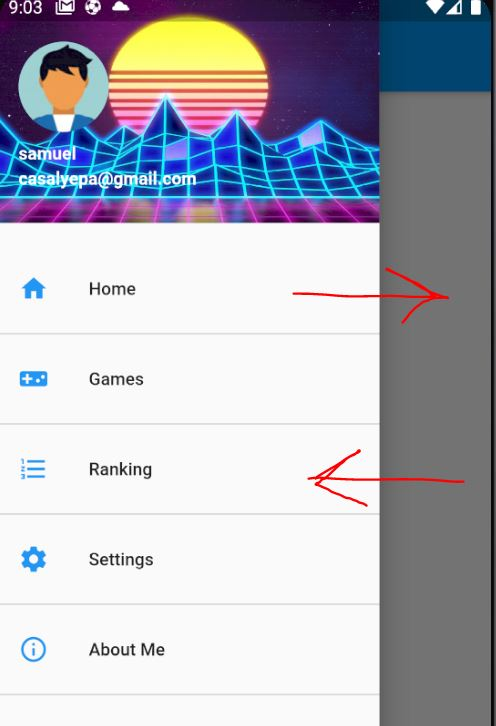
\includegraphics[height=0.8\textwidth]{manual/menuhome.jpg}
	\caption{Menú lateral}\label{fig:menuhome}
\end{figure}
 
Como se aprecia en el menú~\ref{fig:menuhome},  se encuentra la siguiente lista de opciones, dependiendo de cual sea la que se pulse nos redirigirá a la ventana correspondiente:

\begin{itemize}
	\item Home~\ref{fig:homepage}.
	\item Games~\ref{fig:gamespage}.
	\item Ranking~\ref{fig:rankpage}.
	\item Settings~\ref{fig:settingspage}.
	\item About me~\ref{fig:aboutpage}.
\end{itemize}

En el caso de que se quiera salir de la sesión que tenemos abierta, se debe pulsar en nuestra imagen~\ref{fig:mostrarlogout} y aparecerá un cuadro de alerta con las opciones disponibles, se pulsará en \emph{Sign out}~\ref{fig:salir}.

\begin{figure}[H]
	\centering
	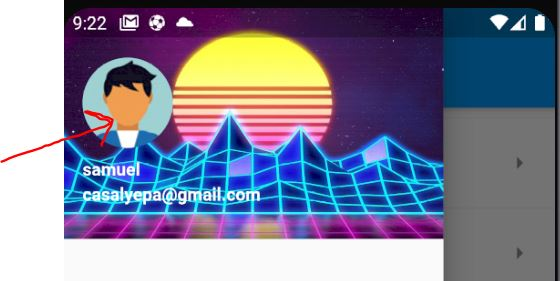
\includegraphics[width=0.7\textwidth]{manual/mostrarlogout.jpg}
	\caption{Mostrar sign out}\label{fig:mostrarlogout}
\end{figure}

\begin{figure}[H]
	\centering
	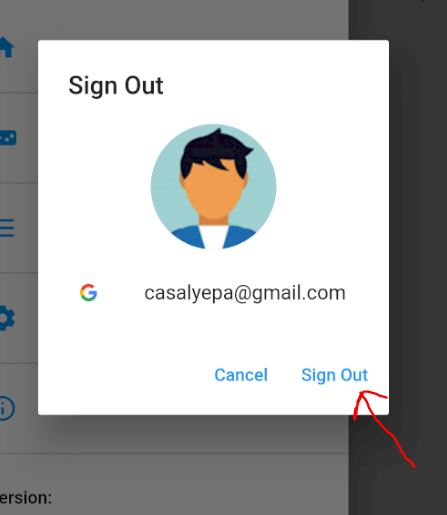
\includegraphics[width=0.7\textwidth]{manual/salir.jpg}
	\caption{Sign Out}\label{fig:salir}
\end{figure}

\subsection{Settings}\label{settings}
Este apartado del menú, es para manejar las opciones referentes a la aplicación, como podemos ver~\ref{fig:settingspage}. Cada una de estas, es un \emph{slider} o deslizador, que si está activado, quiere decir que está a \emph{true} o verdadero.

\begin{figure}[H]
	\centering
	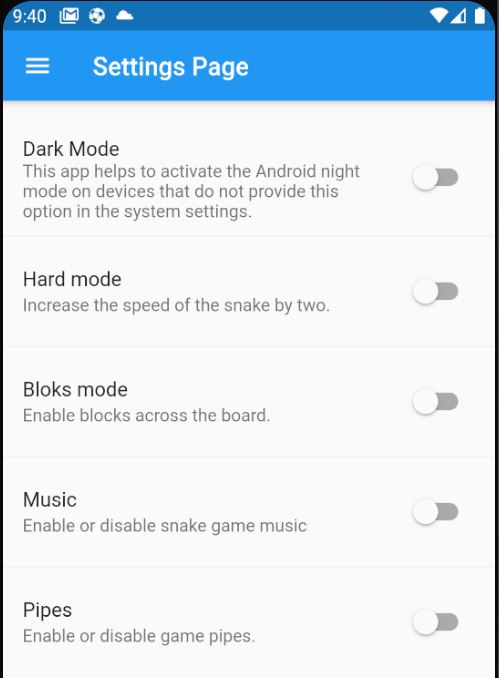
\includegraphics[height=0.8\textwidth]{manual/settings.jpg}
	\caption{Settings}\label{fig:settingspage}
\end{figure}

Una descripción de lo que hacen cada uno de los ajustes:

\begin{itemize}
	\item \textbf{Dark mode:} cambia el color de la aplicación a modo oscuro, con el fin de ahorrar batería o para personas que tengan dificultades visuales~\ref{fig:darkmode}.
	\begin{figure}[H]
		\centering
		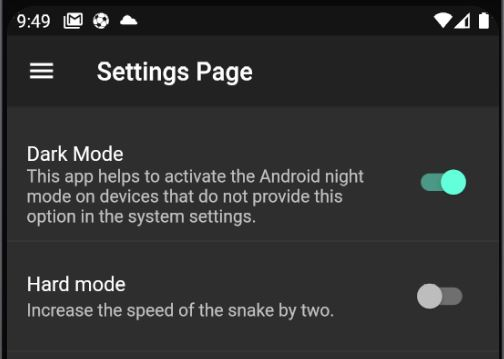
\includegraphics[width=0.8\textwidth]{manual/darkmode.jpg}
		\caption{Dark Mode}\label{fig:darkmode}
	\end{figure}
	\item \textbf{Hard mode:} aumenta la velocidad del snake~\ref{fig:snakepage}, para que sea el doble de rápido.
	\item \textbf{Blocks mode:} reparte bloques a través del tablero del snake~\ref{fig:snakepage}, para tener una dificultad añadida.
	\item \textbf{Music:} habilita o deshabilita la música durante las partidas del snake~\ref{fig:snakepage}.
	\item \textbf{Hard mode:} crea dos tuberías por las cuales la serpiente puede teletransportarse en el tablero, durante el  snake~\ref{fig:snakepage}.
\end{itemize}

\subsection{About me}\label{about}
Pretende mostrar la información referente al creador de la aplicación, como muestra el diseño~\ref{fig:aboutpage}. Se aprecia un \emph{corousel}, con imágenes de los lenguajes de programación conocidos y debajo de dicho elementos, unos icono botones, que enlazan con las páginas de interés.

\begin{figure}[H]
	\centering
	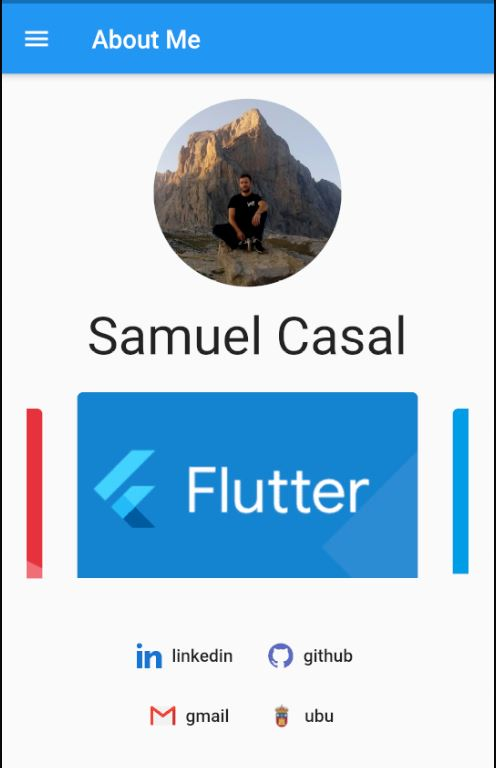
\includegraphics[height=0.7\textwidth]{manual/aboutpage.jpg}
	\caption{About me}\label{fig:aboutpage}
\end{figure}

La lista de \emph{iconbuttons}, con los enlaces:
\begin{itemize}
	\item Linkedin~\cite{linkedin:cuenta}.
	\item Github~\cite{github:repo}.
	\item Gmail~\cite{mailto:mailto}.
	\item Universidad de Burgos~\cite{ubu:page}.
\end{itemize}

Cada una de las opciones abrirá la aplicación correspondiente en el caso de que se encuentre disponible en el terminal, de no ser así se mostrará en el navegador.

En el caso de \emph{Gmail}, nos abre la vista~\ref{fig:mailto}, para mandar un correo al creador de la aplicación, con algún tipo de \emph{feedback}.

\begin{figure}[H]
	\centering
	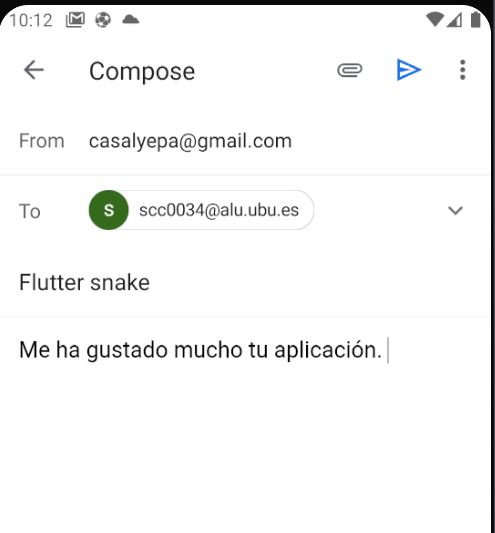
\includegraphics[height=0.9\textwidth]{manual/mailto.jpg}
	\caption{Mail to}\label{fig:mailto}
\end{figure}

\subsection{Menú de juegos}\label{menugames}
En este apartado se muestra una lista con todos los juegos de la colección que están disponibles, la finalidad es que el usuario pueda decidir de una manera sencilla a qué quiere jugar. Por lo que es tan simple como pulsar en la opción correspondiente~\ref{fig:gamespage}.

\begin{figure}[H]
	\centering
	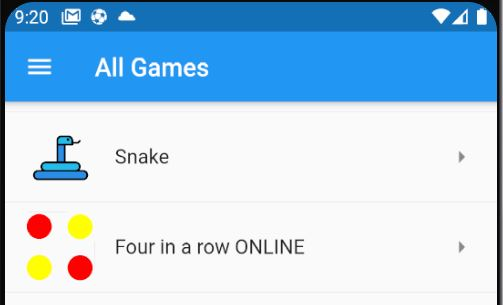
\includegraphics[width=0.7\textwidth]{manual/gamespage.jpg}
	\caption{Games menú}\label{fig:gamespage}
\end{figure}

\subsection{Snake}\label{snake}
Es el juego de la serpiente~\ref{fig:snakepage}. Cuando se entra el juego permanece a la espera hasta que se toca la pantalla (\emph{onTab}). Una vez se produzca esto comienza la serpiente a moverse. El diseño del tablero, depende de las opciones que se tengan seleccionadas en settings~\ref{fig:settingspage}.

El juego consiste en lograr la mayor puntuación posible comiendo lenguajes de programación que están repartidos de forma aleatoria por toda la superficie disponible del tablero.

El marcador de los puntos se encuentra arriba a la derecha de la pantalla.

Los controles de desplazamiento son:
\begin{itemize}
	\item \textbf{Arriba:} deslizamiento vertical superior.
	\item \textbf{Abajo:} deslizamiento vertical inferior.
	\item \textbf{Derecha:} deslizamiento lateral derecho.
	\item \textbf{Izquierda:} deslizamiento lateral izquierdo.
\end{itemize}

Cabe destacar que el menú no está disponible para las ventanas de los juegos, porque puede que se interfiera con la navegabilidad del sistema.

\begin{figure}[H]
	\centering
	
\includegraphics[height=0.9\textwidth]{manual/snake.jpg}
	\caption{Snake game}\label{fig:snakepage}
\end{figure}

El juego finaliza desplegando la ventana~\ref{fig:gameover}, cuando se da una de las siguientes situaciones:
\begin{itemize}
	\item Impacto en la pared que rodea el tablero.
	\item Choque contra uno de los bloques repartidos en la superficie.
	\item No entrar en la tubería por la apertura.
	\item Cabeza de la serpiente choque contra el cuerpo de la misma.
\end{itemize}

\begin{figure}[H]
	\centering
	
\includegraphics[height=0.9\textwidth]{manual/gameover.jpg}
	\caption{Snake game over}\label{fig:gameover}
\end{figure}

Cuando se produce el \emph{game over}~\ref{fig:gameover}, tenemos 3 opciones de las cuales se debe elegir una:

\begin{enumerate}
	\item \textbf{Play Again:} vuelves a jugar la partida con el contador de los puntos a cero.
	\item \textbf{Submit score:} si se da la situación de una mejora de puntuación, con respecto a anteriores partidas, para el jugador que se encuentra logueado, se enviará al formulario~\ref{fig:rankform} de ingreso de datos.
	En el caso de que no tengamos mejora, se puede ver el ranking~\ref{fig:rankpage}.
	
	\begin{figure}[H]
		\centering
		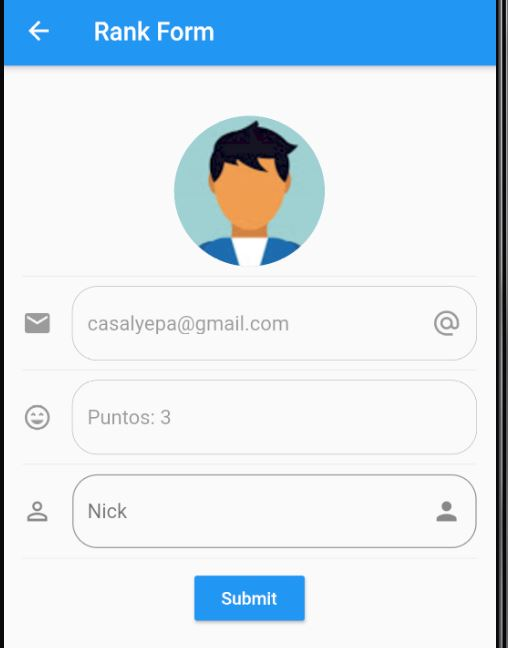
\includegraphics[height=0.9\textwidth]{manual/rankform.jpg}
		\caption{Formulario del ranking}\label{fig:rankform}
	\end{figure}
	
	En el formulario se encuentran el campo de correo y puntuación bloqueadas como medida de seguridad, por lo que se deja la opción de añadir un \emph{nick}. Una vez pulsado el botón de \emph{Submit},se redirigirá a la pantalla de ranking~\ref{fig:rankpage}.
	
	\item \textbf{Video:} permite ver un vídeo para volver a continuar con la partida. Esta opción solo está disponible una vez por juego.
	
		\begin{figure}[H]
		\centering
		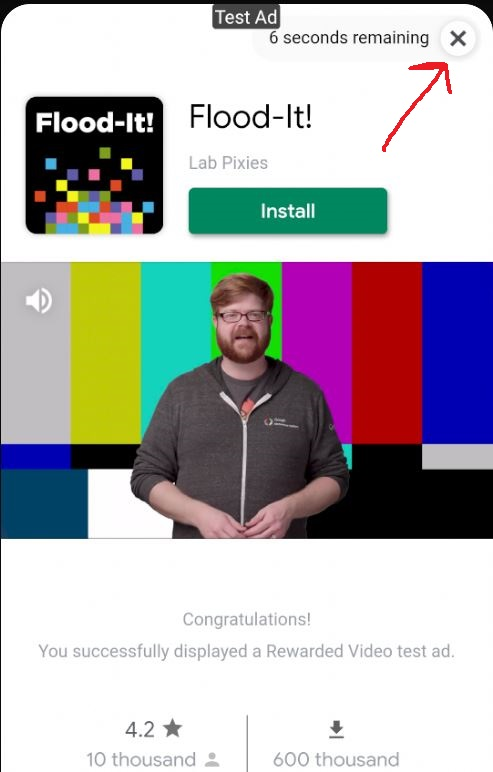
\includegraphics[height=0.7\textwidth]{manual/video.jpg}
		\caption{Vídeo recompensa}\label{fig:video}
		\end{figure}
	
	Es necesario que se permanezcan los segundos indicados para volver a continuar con el juego. 
	
	Tras el impacto. la partida decide que dirección toma la serpiente de forma eficiente para evitar que se produzcan situaciones extrañas.
		
\end{enumerate}

\subsection{Ranking}\label{rank}
Es una clasificación de jugadores, dependiendo de la puntuación lograda en el juego del snake~\ref{fig:snakepage}. Según qué usuario entre a ver el contenido de este~\ref{fig:rankpage}, se verá una línea de color dorado indicando el nivel obtenido.

En el podio de los tres primeros jugadores aparecerá una insignia en forma de medalla, destacando el logro conseguido.

\begin{figure}[H]
	\centering
	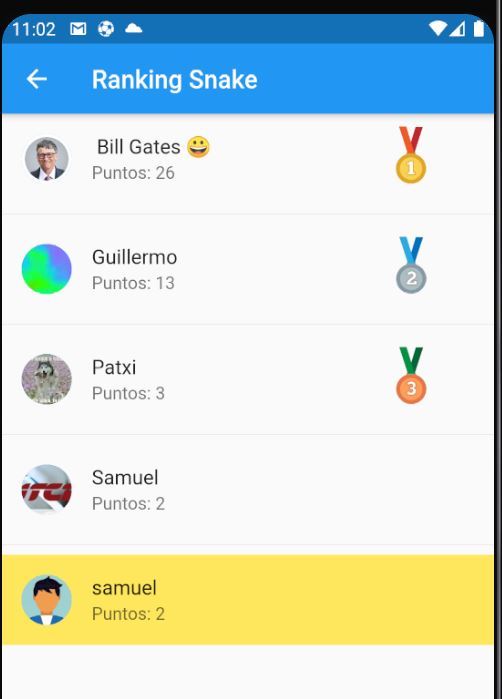
\includegraphics[height=0.8\textwidth]{manual/rankpage.jpg}
	\caption{Ranking}\label{fig:rankpage}
\end{figure}

\subsection{Menú juego cuatro en raya online}\label{cuatromenu}
Es la pantalla inicial del juego~\ref{fig:cuatromenu}, ya que siendo en modo online, uno de los jugadores debe de ser el creador de la  partida (\emph{invite friend}) y el otro el que se una a la partida creada (\emph{join game}).

Por lo que se encuentran dos botones que redirigen a:
\begin{itemize}
	\item Invitar a un amigo~\ref{fig:cuatroinvitar}.
	\item Unirse a una partida creada~\ref{fig:cuatrounir}.
\end{itemize}

\begin{figure}[H]
	\centering
	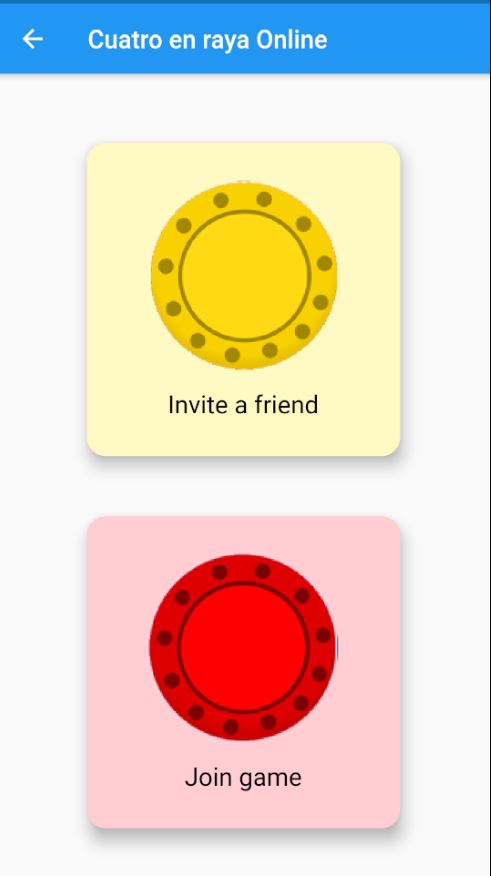
\includegraphics[height=0.7\textwidth]{manual/cuatromenu.jpg}
	\caption{Menú del cuatro en raya}\label{fig:cuatromenu}
\end{figure}

\subsubsection{Invitar}\label{cuatroinvitar}
Cuando se entra en la pantalla, se genera una clave única, que es necesaria para hacer la conexión por parte del invitado. Para ello hay un botón \emph{share} que facilita el compartir la \emph{key}.

Hay disponible un botón de volver, que lo que hace es destruir la clave para salir a la pantalla anterior~\ref{fig:cuatromenu}. Es el mismo efecto que si se da a la pestaña de volver atrás.


\begin{figure}[H]
	\centering
	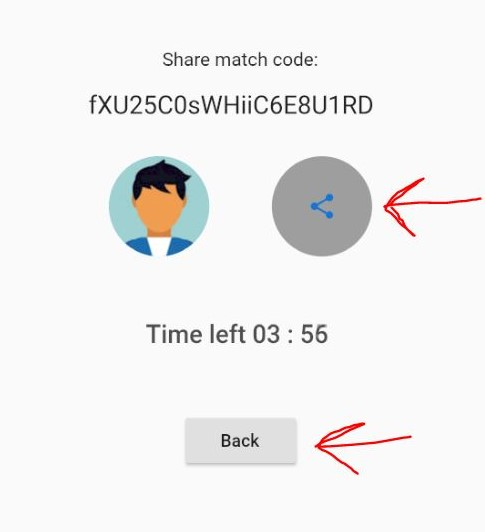
\includegraphics[height=0.7\textwidth]{manual/invite.jpg}
	\caption{Invitar cuatro en raya}\label{fig:cuatroinvitar}
\end{figure}

\begin{figure}[H]
	\centering
	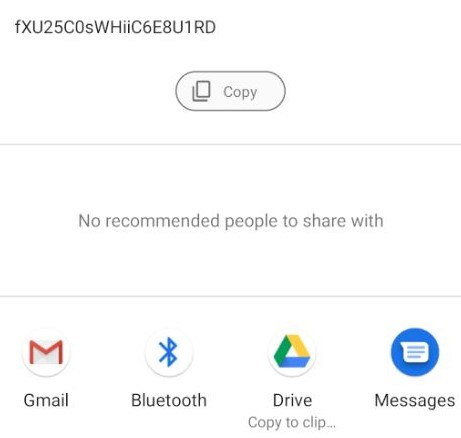
\includegraphics[width=0.6\textwidth]{manual/sharegame.jpg}
	\caption{Compartir clave}\label{fig:sharegame}
\end{figure}

Cuando se pulsa en el botón de compartir aparece un cuadro de diálogo~\ref{fig:sharegame} mostrando las aplicaciones que facilitan el envío de la clave.

En el caso de que el contador del tiempo restante \emph{time left}, llegue a cero es porque se da por hecho que no se recibe respuesta por parte del invitado, saliendo el cuadro de diálogo~\ref{fig:noplayerfound}.

\begin{figure}[H]
	\centering
	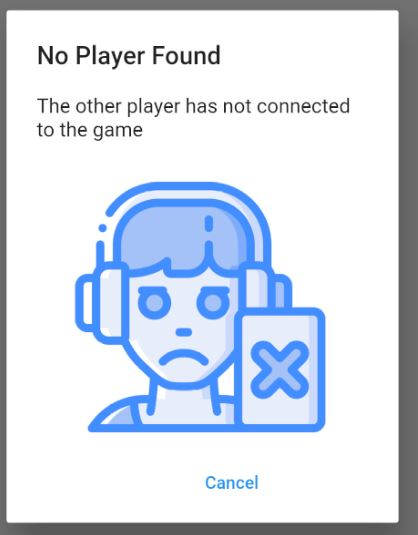
\includegraphics[width=0.6\textwidth]{manual/noplayerfound.jpg}
	\caption{Sin jugador}\label{fig:noplayerfound}
\end{figure}

\subsubsection{Unir}\label{cuatrounir}
Pantalla con un formulario de entrada de datos~\ref{fig:cuatrounir}, se usa para escribir la clave recibida por parte del compañero o amigo. 

Si se da la situación de que no es la clave correcta se avisará por pantalla~\ref{fig:uniralert}.

En el caso de que tengamos una clave válida, se redirigirá hacia la pantalla del juego~\ref{fig:cuatrojuego}.

\begin{figure}[H]
	\centering
	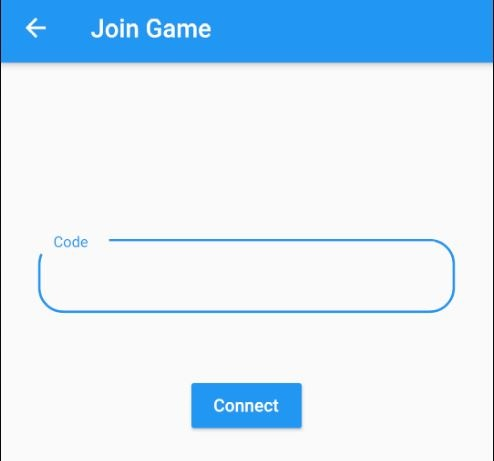
\includegraphics[width=0.7\textwidth]{manual/joingame.jpg}
	\caption{Formulario para unirse a partida}\label{fig:cuatrounir}
\end{figure}

\begin{figure}[H]
	\centering
	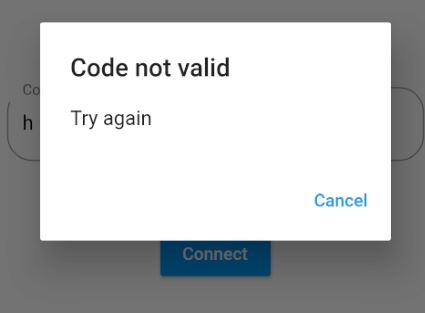
\includegraphics[width=0.7\textwidth]{manual/uniralert.jpg}
	\caption{Alerta de clave no válida}\label{fig:uniralert}
\end{figure}

\subsubsection{Juego}\label{cuatrojuego}
Página con el contenido del juego~\ref{fig:cuatrojuego}. Este consiste en formar líneas de longitud cuatro, en cualquiera de las direcciones posibles: diagonal, vertical y horizontal. Nada más entrar en esta pantalla, se produce el sorteo, para saber quién de los dos participantes comienza a jugar~\ref{fig:sorteo}.

\begin{figure}[H]
	\centering
	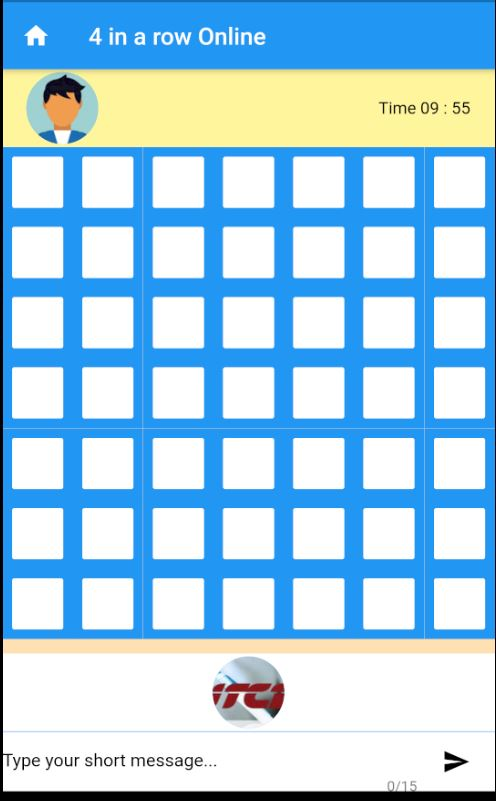
\includegraphics[height=0.9\textwidth]{manual/cuatrojuego.jpg}
	\caption{Cuatro en raya}\label{fig:cuatrojuego}
\end{figure}

\begin{figure}[H]
	\centering
	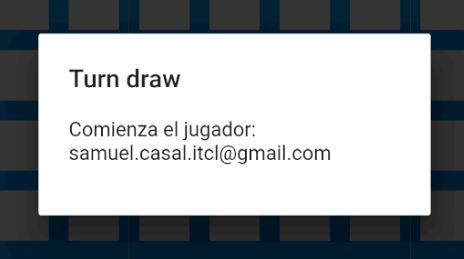
\includegraphics[width=0.8\textwidth]{manual/turno.jpg}
	\caption{Sorteo del turno}\label{fig:sorteo}
\end{figure}

La distribución de la pantalla~\ref{fig:cuatrojuego} es la siguiente, comenzando por la parte de arriba hasta abajo:

\begin{itemize}
	\item Cabecera superior~\ref{fig:cabecera}, se encuentra el rival a batirse, representado mediante una imagen, siendo esta la de la cuenta de \emph{Google}. Dependiendo del color de fondo, se indica si está en su turno o no.
	
	En la parte central hay un espacio para mostrar los mensajes recibidos por parte del contrincante.
	
	En la parte lateral derecha se encuentra el contador del tiempo transcurrido.
	
	 \begin{figure}[H]
	 	\centering
	 	
\includegraphics[width=0.8\textwidth]{manual/cabecera.jpg}
	 	\caption{Zona superior}\label{fig:cabecera}
	 \end{figure}
 
	\item En la parte central~\ref{fig:tablero} se dispone el tablero de siete filas por siete columnas. En el caso de que sea nuestro turno, se debe pinchar en la pantalla, donde sea posible colocar una ficha, es decir, que si debajo de la celda se encuentra vacío no será posible colocar la ficha y se deberá proceder a buscar otro sito en el que se pueda.
	
	\begin{figure}[H]
		\centering
		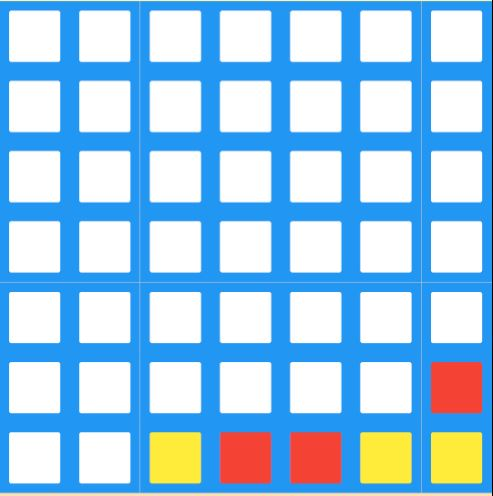
\includegraphics[width=0.8\textwidth]{manual/tablero.jpg}
		\caption{Tablero}\label{fig:tablero}
	\end{figure}

	\item En la parte inferior~\ref{fig:inferior}, se encuentra la imagen del aliado, es decir, puede ser el jugador que se unió o que creó la partida, dependiendo de quién sea el que haya tomado ese rol.
	
	Si esta zona se encuentra con el color de fondo distinto de blanco indica que es el turno de este jugador.
	
	\begin{figure}[H]
		\centering
		
\includegraphics[width=0.8\textwidth]{manual/inferior.jpg}
		\caption{Zona personal}\label{fig:inferior}
	\end{figure}

	\item Campo para introducir mensajes~\ref{fig:mensaje}, está limitado a 15 caracteres, ya que está destinado para mensajes breves o emoticonos.
	
	A la derecha de este campo, se encuentra el botón de enviar. Una vez se envía el mensaje, este se deshabilita, para no saturar la línea. Pasados 10 segundos volverá a estar operativo.
	
	\begin{figure}[H]
		\centering
		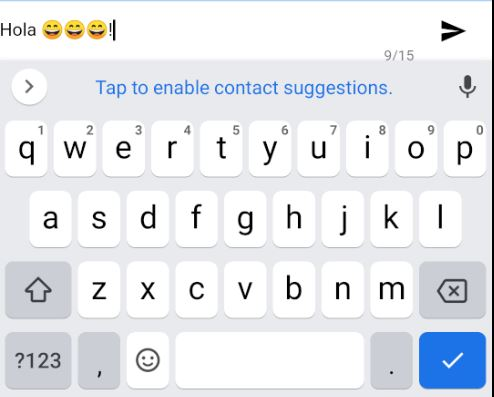
\includegraphics[width=0.8\textwidth]{manual/mensaje.jpg}
		\caption{Envío de mensaje}\label{fig:mensaje}
	\end{figure}
\end{itemize}

En el momento en que se da la situación de fin de juego, salta la alerta para mostrar quién de los dos jugadores es el ganador de la partida, como se puede ver en la imagen siguiente~\ref{fig:finalcuatro}

\begin{figure}[H]
	\centering
	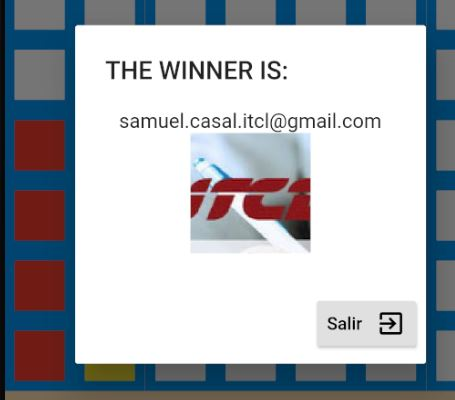
\includegraphics[width=0.8\textwidth]{manual/winer.jpg}
	\caption{Final del cuatro en raya}\label{fig:finalcuatro}
\end{figure} 